
\documentclass[12pt]{article}

% Packages
\usepackage[utf8]{inputenc}
\usepackage{graphicx}        
\usepackage{array}
\usepackage{booktabs}
\usepackage{amsmath, amssymb} 
\usepackage{geometry}        
\usepackage{setspace}        
\usepackage{multirow}
\usepackage{hyperref}        
\usepackage{cite}            
\usepackage{caption}                  
\usepackage{tikz}
\usetikzlibrary{positioning}
\usetikzlibrary{arrows.meta}
\usepackage[utf8]{inputenc}
\usepackage{cite} % For bibliography
\usepackage{setspace} % For spacing if needed
\usepackage{geometry} % Page layout
\geometry{margin=1in}
\usepackage{float}
%\usepackage{tikz-uml}


% Page Setup
\geometry{margin=1in}
\setstretch{1.25}

% Title Info
\title{Milestone 1: Project Foundation \\ \large Modeling and Simulation}
\author{Amaya McCullough}
\date{September 10, 2025}

\begin{document}

\maketitle
\tableofcontents
\newpage

% -----------------------------
\section{Project Proposal}
\subsection{Introduction}

Hospitals face challenges in managing limited bed capacity, especially during demand surges. 
This project uses discrete-event simulation to model a simplified hospital ward where patients arrive randomly, request beds, and receive treatment. 
Patients are prioritized based on severity, reflecting real-world triage. 
The simulation explores how system performance changes under different scenarios, providing insights into resource management and patient flow.

This project develops a discrete-event simulation of hospital bed allocation using Python and the SimPy library. 
The model represents patient arrivals, queueing, and treatment under limited capacity, with patients prioritized by severity. 
Experiments test the impact of varying bed capacity, arrival rates, severity distributions, and treatment times. 
Key performance measures include patient wait times, queue length, and bed utilization. 
Findings highlight trade-offs between efficiency, fairness, and resource use, with implications for hospital resource planning.



\subsection{Objectives}
The main objectives of this project are:
\begin{itemize}
    \item To design and implement a discrete-event simulation model of hospital bed allocation using Python and SimPy.
    \item To analyze patient flow dynamics, including arrivals, waiting times, queue lengths, and bed utilization.
    \item To evaluate system performance under different scenarios of patient demand and bed availability.
    \item To identify potential strategies for improving efficiency and reducing patient wait times during demand surges.
    \item To provide actionable insights that can assist hospital administrators in capacity planning and resource allocation.
\end{itemize}

\subsection{Scope and Limitations}


The scope of this project focuses on simulating hospital bed allocation for a single hospital unit. Patients are classified into three severity levels --- critical, moderate, and mild --- and are assigned priority accordingly. The simulation models patient arrivals, bed requests, treatment times, and discharges.

However, the project has several limitations:
\begin{itemize}
    \item It does not model inter-hospital transfers or staffing constraints such as nurse availability.
    \item The patient arrival process assumes a Poisson distribution and does not account for external factors such as epidemics or policy changes.
    \item Treatment times are assumed to follow a uniform distribution and do not vary by patient condition beyond severity.
    \item The model focuses on short-term operational decision-making rather than long-term planning.
\end{itemize}

\subsection{Methodology}

The project methodology consists of the following steps:

\begin{enumerate}
    \item \textbf{Problem Definition:} Clearly define the hospital bed allocation problem and identify key system components, including patients, beds, and service processes.
    \item \textbf{Model Design:} Develop a conceptual model using UML class and sequence diagrams to represent patient flows and resource interactions.
    \item \textbf{Implementation:} Translate the conceptual model into a Python-based simulation using the SimPy library.
    \item \textbf{Scenario Design:} Define multiple test scenarios, such as baseline, high demand, and increased bed capacity.
    \item \textbf{Experimentation:} Run the simulation for each scenario, collecting data on waiting times, queue lengths, and utilization.
    \item \textbf{Analysis and Reporting:} Analyze the results using statistical methods and visualize findings using plots and summary tabless.
\end{enumerate}
% -----------------------------
\section{Literature Review}

Efficient hospital bed allocation is a longstanding challenge in healthcare operations research. Simulation-based methods have proven effective in capturing the inherent uncertainty of patient arrivals, treatment times, and discharge delays. This section reviews existing work on hospital simulation, queueing models, and resource allocation strategies, highlighting their relevance to the proposed project.

\subsection{Hospital Simulation Models}
Jun et al.~\cite{jun1999simulation} provide a comprehensive survey of simulation in healthcare, emphasizing its ability to model complex, stochastic systems. Their work establishes simulation as a valuable tool for analyzing patient flow and testing operational improvements without disrupting real-world services. This foundational perspective supports the choice of simulation as the methodology for this project.

\subsection{Queueing Theory in Patient Flow}
Green~\cite{green2006queueing} explores queueing models in healthcare, particularly the use of $M/M/c$ systems to analyze waiting times and service capacity. Applying such models to emergency and non-emergency admissions directly informs the design of the hospital bed simulation, where patients compete for limited beds.

\subsection{Bed Allocation and Capacity Management}
Belciug and Gorunescu~\cite{belciug2015learning} present intelligent methods for hospital resource allocation, combining machine learning with simulation to optimize bed usage. Their findings highlight how predictive modeling can reduce overcrowding, which motivates the inclusion of utilization tracking in the proposed simulation.

\subsection{Emergency Department Simulation}
Sinreich and Marmor~\cite{sinreich2005emergency} analyze emergency department operations using discrete-event simulation. Their results demonstrate the importance of prioritization mechanisms for urgent patients. This aligns with the project’s priority scheduling component, ensuring that emergency admissions receive preferential access to beds.

\subsection{Resource Utilization and System Performance}
Fomundam and Herrmann~\cite{fomundam2007survey} survey healthcare supply chain modeling, noting the critical role of capacity utilization in improving efficiency. Their emphasis on measuring throughput and bottlenecks supports the inclusion of performance metrics such as utilization rates and queue lengths in the simulation.

\subsection{Recent Developments}
A recent study by Vanbrabant et al.~\cite{vanbrabant2019simulation} investigates simulation-based hospital admission control policies under uncertain demand. Their results underscore the value of dynamic, data-driven policies over static allocation rules, reinforcing the novelty of capturing emergent behaviors within the proposed system.

\subsection{Summary}
The reviewed literature demonstrates the effectiveness of simulation and queueing models in healthcare operations. While prior studies address aspects of patient flow, bed allocation, and prioritization, the proposed project is distinctive in integrating these components within a single simulation framework. By combining stochastic arrivals, priority-based scheduling, and resource utilization analysis, the project aims to provide a comprehensive tool for understanding and improving hospital bed management.


% -----------------------------
\section{System Design (UML Diagrams)}
\subsection{Use Case Diagram}

\begin{figure}[h]
\centering
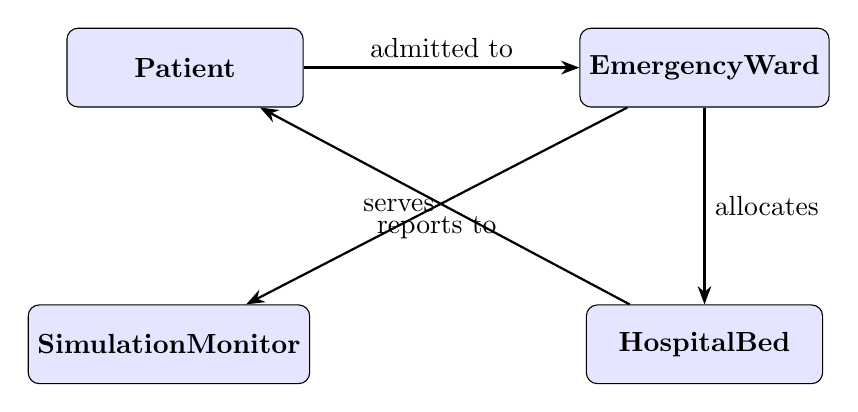
\begin{tikzpicture}[
    class/.style={rectangle, draw, rounded corners, minimum width=3cm, minimum height=1cm, fill=blue!10, font=\bfseries}
]

% Classes
\node[class] (patient) {Patient};
\node[class, right=3.5cm of patient] (ward) {EmergencyWard};
\node[class, below=2.5cm of ward] (bed) {HospitalBed};
\node[class, left=3.5cm of bed] (monitor) {SimulationMonitor};

% Relationships
\draw[-Stealth, thick] (patient) -- (ward) node[midway, above] {admitted to};
\draw[-Stealth, thick] (ward) -- (bed) node[midway, right] {allocates};
\draw[-Stealth, thick] (ward) -- (monitor) node[midway, below] {reports to};
\draw[-Stealth, thick] (bed) -- (patient) node[midway, left] {serves};

\end{tikzpicture}
\caption{Class diagram for hospital simulation.}
\end{figure}

\subsection{Class Diagram}
\begin{figure}[h]
\centering
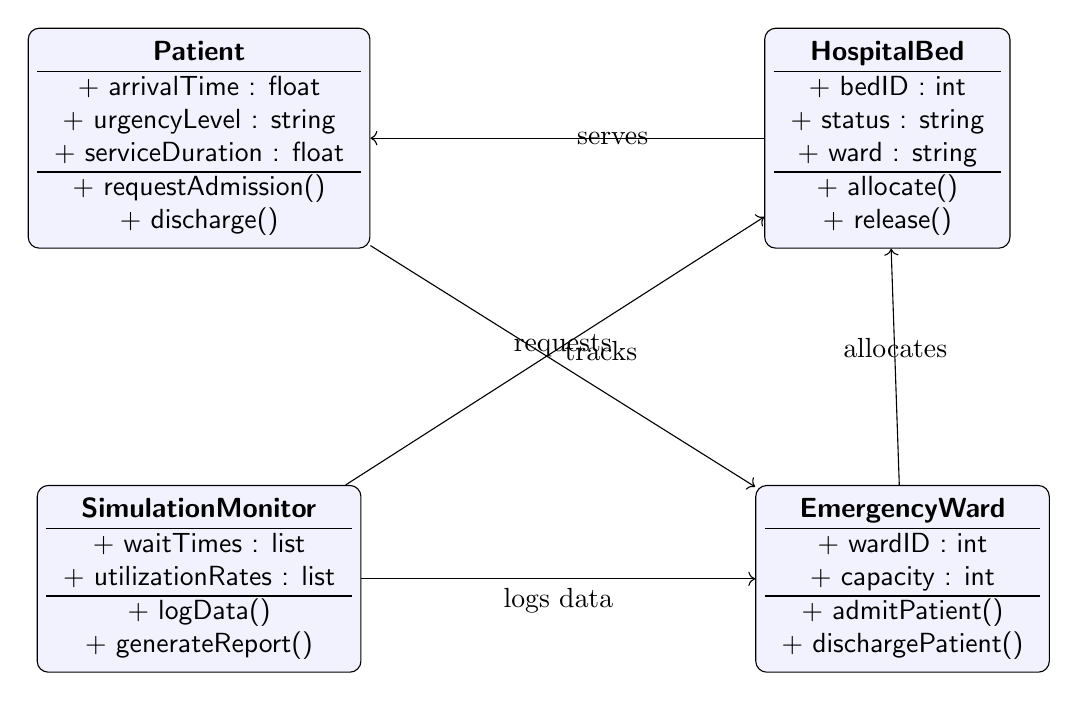
\begin{tikzpicture}[
  class/.style={rectangle, draw, fill=blue!5, rounded corners, minimum width=3cm, font=\sffamily}
]

% Classes
\node[class] (patient) {
\begin{tabular}{c}
  \textbf{Patient}\\
  \hline
  + arrivalTime : float \\
  + urgencyLevel : string \\
  + serviceDuration : float \\
  \hline
  + requestAdmission() \\
  + discharge()
  \end{tabular}
};

\node[class, right=5cm of patient] (bed) {
\begin{tabular}{c}
  \textbf{HospitalBed}\\
  \hline
  + bedID : int \\
  + status : string \\
  + ward : string \\
  \hline
  + allocate() \\
  + release()
  \end{tabular}
};

\node[class, below=3cm of patient] (monitor) {
\begin{tabular}{c}
  \textbf{SimulationMonitor}\\
  \hline
  + waitTimes : list \\
  + utilizationRates : list \\
  \hline
  + logData() \\
  + generateReport()
  \end{tabular}
};

\node[class, right=5cm of monitor] (ward) {
\begin{tabular}{c}
  \textbf{EmergencyWard}\\
  \hline
  + wardID : int \\
  + capacity : int \\
  \hline
  + admitPatient() \\
  + dischargePatient()
  \end{tabular}
};

% Relationships
\draw[->] (patient) -- node[midway, above] {requests} (ward);
\draw[->] (ward) -- node[midway, above] {allocates} (bed);
\draw[->] (bed) -- node[midway, right] {serves} (patient);
\draw[->] (monitor) -- node[midway, below] {logs data} (ward);
\draw[->] (monitor) -- node[midway, right] {tracks} (bed);

\end{tikzpicture}
\caption{UML Class Diagram: Hospital Bed Simulation}
\end{figure}

\subsection{Sequence Diagram (Optional)}

\begin{figure}[H]
\centering
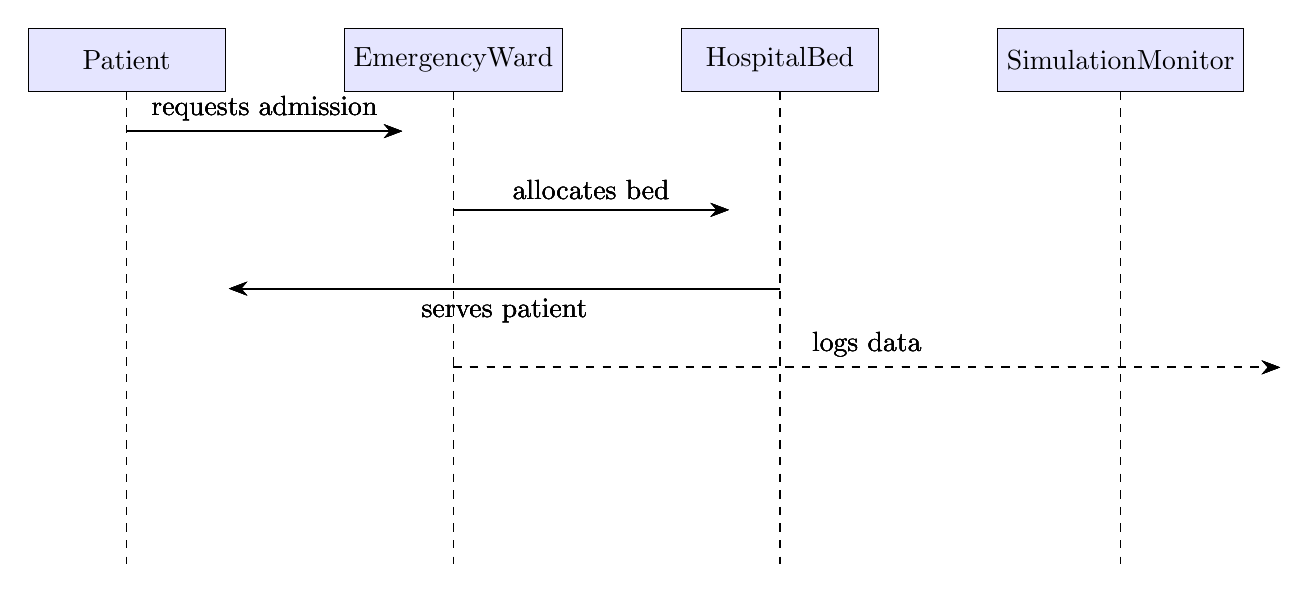
\begin{tikzpicture}[
    lifeline/.style={rectangle, draw, minimum width=2.5cm, minimum height=0.8cm, fill=blue!10},
    msg/.style={-Stealth, thick},
    dashedmsg/.style={dashed, -Stealth, thick}
]
% Lifelines (top row)
\node[lifeline] (patient) {Patient};
\node[lifeline, right=1.5cm of patient] (ward) {EmergencyWard};
\node[lifeline, right=1.5cm of ward] (bed) {HospitalBed};
\node[lifeline, right=1.5cm of bed] (monitor) {SimulationMonitor};

% Vertical lifeline dashed lines
\foreach \x in {patient, ward, bed, monitor} {
   \draw[dashed] (\x.south) -- ++(0,-6);

% Messages
\draw[msg] (patient.south) ++(0,-0.5) -- ++(3.5,0) node[midway, above] {requests admission};
\draw[msg] (ward.south) ++(0,-1.5) -- ++(3.5,0) node[midway, above] {allocates bed};
\draw[msg] (bed.south) ++(0,-2.5) -- ++(-7,0) node[midway, below] {serves patient};
\draw[dashedmsg] (ward.south) ++(0,-3.5) -- ++(10.5,0) node[midway, above] {logs data};
}

\end{tikzpicture}
\caption{Sequence diagram for hospital simulation.}
\end{figure}

% -----------------------------
\section{Conclusion}
Summarize the proposed project and expected outcomes.
This project proposed the design and implementation of a discrete-event simulation model to study hospital bed allocation under conditions of limited capacity and variable patient demand. By modeling patient arrivals, severity levels, and treatment durations, the simulation provides a realistic representation of how hospital resources are utilized over time. 

The model enables experimentation with different allocation policies, allowing stakeholders to evaluate strategies for improving patient flow, reducing wait times, and optimizinf bed utilization. Additionally, the simulation incorporates data logging and reporting features, which support further analysis of system performance.

\textbf{Expected outcomes} of this project include identifying key factors that contribute to botttlenecks in patient care, providing insights into the impact of prioritization rules, and offering data-driven recommendations for hospital resource management. The final results will help heaLthcare administrators make informed decisions to enhance operational efficiency and improve patient outcomes. 

% -----------------------------

\newpage
% Bibliography
\bibliographystyle{IEEEtran}
%\bibliographystyle{plain}
\bibliography{references}

\end{document}
